\ifdefined\PTDAuthorVersion
  \documentclass[sigconf,natbib=true]{acmart}
\else
  \documentclass[sigconf,natbib=true,anonymous=true]{acmart}
\fi

\usepackage{amsmath,booktabs,tabularx}
\usepackage{algorithm}
\usepackage{algpseudocode}
\usepackage{tikz}
\usepackage{placeins}
\usetikzlibrary{arrows.meta,positioning}

\setcopyright{none}
\settopmatter{printacmref=false,printccs=true,printfolios=true}
\renewcommand\footnotetextcopyrightpermission[1]{}
\acmConference[SIGIR '27]{The 50th International ACM SIGIR Conference on Research and Development in Information Retrieval}{July 18--24, 2027}{San Jose, CA, USA}
\acmYear{2027}

\newcommand{\ptd}{\textsc{PTD}}
\newcommand{\pending}[1]{\textbf{[Pending: #1]}}

\title{From Ranking to Retrieval: Purchase-Aware Tree Distillation for Recommendation}

% The review build suppresses this identity; main-author.tex displays it.
% Given name: Naoyuki; family name: Tomita.
\author{Naoyuki Tomita}
\ifdefined\PTDAuthorVersion
  \affiliation{%
    \institution{X Pipelines Co., Ltd.}
    \city{Ho Chi Minh City}
    \country{Vietnam}
  }
\else
  \affiliation{\institution{Affiliation withheld for anonymous review}}
\fi

\begin{abstract}
Large-scale home feeds commonly separate candidate retrieval from a purchase-oriented ranker. This division creates an objective gap: a retriever is optimized from sparse interactions while the downstream ranker estimates a denser purchase utility. We formulate Purchase-aware Tree Distillation (\ptd), a preregistered utility-projection method for a balanced item tree. A frozen Entire Space Multi-Task Model (ESMM) supplies item purchase log-odds at leaf decisions; for each internal child, \ptd{} sums the purchase utility of eligible descendant items and normalizes the resulting masses across siblings. The resulting targets supervise the local decisions traversed by the tree, without an online teacher call. \ptd{} also includes an HSTU-style action-sequence encoder and a train-only alternating tree update related to TDM/JTM. The evaluation contract fixes a point-in-time-safe evidence universe, a five-date temporal test, three random seeds, paired user bootstrap inference, and explicit quality, diversity, and latency guardrails. A verified legacy artifact establishes the common evidence universe and teacher anchor (12,844,800 test pairs; ESMM purchase NDCG@50 0.17626), but it contains no \ptd{} result. The prospective five-day tree-family results are pending; consequently this draft makes no efficacy or priority claim. The accompanying artifact provides schemas, a claim--evidence ledger, deterministic table/figure generation, and fail-closed validation so that empirical claims can be promoted only after immutable manifests, hashes, and evaluation JSON are available.
\end{abstract}

\ccsdesc[500]{Information systems~Recommender systems}
\ccsdesc[500]{Information systems~Retrieval models and ranking}
\ccsdesc[300]{Computing methodologies~Knowledge representation and reasoning}

\keywords{candidate retrieval, recommender systems, tree-based retrieval, knowledge distillation, conversion modeling, sequential recommendation}

\begin{document}
\maketitle

\section{Introduction}
Industrial recommendation pipelines must retrieve a small candidate set before an expressive ranker can evaluate it. Two-tower retrieval makes this stage compatible with maximum-inner-product indexes, but constrains the interaction function. Tree-based deep models instead place items at leaves and evaluate user--node compatibility from root to leaf, supporting expressive scorers with logarithmic dependence on corpus size under fixed branching and beam assumptions~\citep{zhu2018tdm}. Their supervision, however, is usually derived from observed positive paths and sampled negatives. The downstream purchase ranker may encode a richer ordering than those binary path labels.

This paper studies a deliberately narrow question: can a fixed purchase model teach the local decisions made by a tree retriever? We call the registered method Purchase-aware Tree Distillation (\ptd). The teacher is a frozen ESMM-style model whose purchase score factors as predicted click-through rate times predicted post-click conversion rate~\citep{ma2018esmm}. The teacher natively scores items in a flat candidate space, whereas the student must decide which child to traverse at each level. \ptd{} bridges that structural mismatch by projecting item utility onto sibling-conditional targets: leaves retain purchase log-odds, and internal children receive the aggregate purchase mass of their eligible descendants. This supplies routing supervision before the target item is reached and avoids requiring a globally normalized teacher distribution over the complete catalog. The resulting mechanistic hypothesis is falsifiable: under a fixed finite beam, the subtree aggregation rule---not merely the presence of distillation---may determine whether high-utility items survive early pruning.

Three components are integrated. First, an HSTU-style encoder represents the user's point-in-time action sequence~\citep{zhai2024hstu}. Second, a balanced tree constrains serving work and makes sibling groups explicit. Third, an optional JTM-style alternating phase updates item assignments from training evidence only and locks the tree before test scoring~\citep{zhu2019jtm}. Figure~\ref{fig:architecture} summarizes the design.

This is an evidence-bounded draft. We contribute (i) an applied formulation that combines purchase-oriented ranker supervision with tree-induced marginalization to train the internal and leaf decisions of an explicit candidate retriever, (ii) a preregistered temporal evaluation and ablation plan, and (iii) a reproducible artifact contract that separates verified, preregistered, and pending statements. Factorized and marginal structural distillation, ranker-to-retriever transfer, conversion-aware candidate generation, and beam-aware training all have precedents. We therefore make no ``first'' claim and do not claim that \ptd{} improves retrieval before the prospective evaluation passes the evidence gate.

\begin{figure*}[t]
\centering
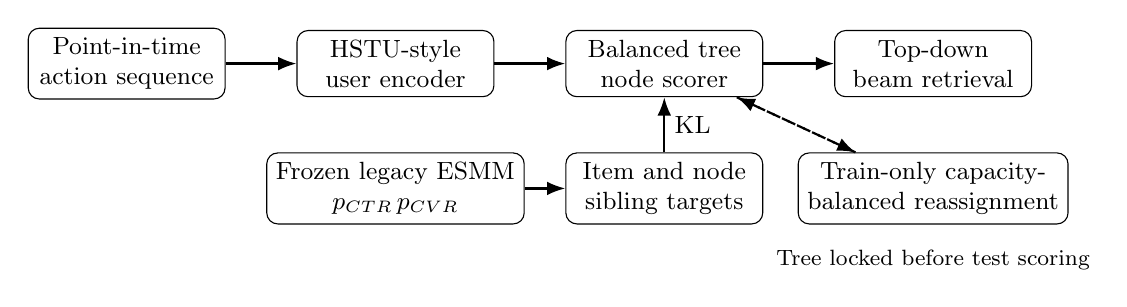
\begin{tikzpicture}[node distance=7mm and 9mm, every node/.style={font=\small}, box/.style={draw,rounded corners,align=center,minimum height=8mm,minimum width=25mm}, arr/.style={-Latex,thick}]
\node[box] (seq) {Point-in-time\\action sequence};
\node[box,right=of seq] (hstu) {HSTU-style\\user encoder};
\node[box,right=of hstu] (tree) {Balanced tree\\node scorer};
\node[box,right=of tree] (beam) {Top-down\\beam retrieval};
\node[box,below=of hstu] (teacher) {Frozen legacy ESMM\\$p_{CTR}\,p_{CVR}$};
\node[box,below=of tree] (siblings) {Item and node\\sibling targets};
\node[box,below=of beam] (alt) {Train-only capacity-\\balanced reassignment};
\draw[arr] (seq) -- (hstu);
\draw[arr] (hstu) -- (tree);
\draw[arr] (tree) -- (beam);
\draw[arr] (teacher) -- (siblings);
\draw[arr] (siblings) -- node[right]{KL} (tree);
\draw[arr,dashed] (tree) -- (alt);
\draw[arr,dashed] (alt) -- (tree);
\node[align=center,below=2mm of alt,font=\footnotesize] {Tree locked before test scoring};
\end{tikzpicture}
\caption{Registered PTD design. Solid arrows are model/data flow; dashed arrows occur only during train-side alternating optimization. The teacher is frozen.}
\label{fig:architecture}
\end{figure*}


\section{Problem Formulation}
Let $u$ denote a request with a history $H_u$ available strictly before snapshot time $t$, and let $\mathcal{I}_t$ be eligible items. A balanced $b$-ary tree $\mathcal{T}$ maps each item $i$ to a leaf. At depth $h$, beam search keeps $B$ nodes according to a student score $s_\theta(u,n)$. The serving objective is to retrieve a set $R_K(u)$ with high future purchase utility while bounding the number of node evaluations.

Write the root-to-leaf code for item $i$ as $\pi_{\mathcal{T}}(i)=(n_0,\ldots,n_H)$ and the children competing with $n_h$ as $S_h(i)$. With a balanced tree, $H=\lceil\log_b |\mathcal{I}_t|\rceil$ up to capacity padding. The HSTU-style variant encodes the user once, after which beam retrieval evaluates at most $b+B b(H-1)$ child nodes before leaf truncation, or $O(BbH)$ scorer calls; the node-conditioned DIN ablation is timed separately. This bound motivates a local decision objective: the student need only order siblings encountered by the beam, rather than score every eligible item online.

For each eligible pair, the frozen teacher produces
\begin{equation}
q_T^{\mathrm{purchase}}(u,i)
= \widehat{p}_{T}(\mathrm{click}\mid u,i)
  \widehat{p}_{T}(\mathrm{purchase}\mid \mathrm{click},u,i),
\label{eq:teacher}
\end{equation}
following the ESMM factorization. This score is a training signal, not ground truth. It can inherit calibration, exposure, and representation biases from the legacy model.

The observed label $y_{ui}$ is one only when a home-feed click-to-purchase event occurs in $[t,t+24\mathrm{h})$. All sequence, item, teacher-feature, and tree-construction inputs must precede $t$. Our primary metric is macro user purchase NDCG@50 over users with an observed purchase.

\section{Purchase-aware Tree Distillation}
\subsection{Point-in-time HSTU-style user encoder}
The frozen input contains separate click and purchase product-ID streams, each most-recent-first and capped at 30. It does not retain per-event timestamps or a total order across streams. We reverse each stream independently to oldest-to-newest and apply the same two-layer, four-head, 64-dimensional gated sequential-transduction stack to both. Item and stream-type embeddings are shared, positional encoding is learned, and time encoding is disabled. Final non-padding click and purchase states are fused with a hashed-user state into $z_u$; empty streams use a learned token. We use ``HSTU-style'' because the component adopts gated sequential transduction, not because it reproduces the scale or complete feature set of \citet{zhai2024hstu}. A node representation and contextual features enter $s_\theta(z_u,e_n,x_{un})$.

The registered non-HSTU ablation consumes exactly the same two streams and embeddings through per-stream multiwindow DIN operators with windows $(1,2,3,4,5,5,10)$. It shares the tree, scorer head, optimizer, examples, and width, but exact parameter equality is not claimed; trainable counts and measured latency are mandatory outputs. Thus RQ4 compares two fixed sequence operators without inventing unavailable temporal evidence.

\subsection{Sibling teacher distributions}
For a leaf-parent sibling set $S_i$, item-level teacher logits are
\begin{equation}
a_T(u,j)=\operatorname{logit}\!\left(
\operatorname{clip}(q_T^{\mathrm{purchase}}(u,j),\epsilon,1-\epsilon)
\right), \quad j\in S_i.
\end{equation}
For an internal child $c$, the teacher mass aggregates eligible descendant items from the training candidate universe,
\begin{equation}
m_T(u,c)=\sum_{j\in \operatorname{desc}(c)\cap C_u}
q_T^{\mathrm{purchase}}(u,j),
\end{equation}
and sibling logits are $a_T(u,c)=\log(m_T(u,c)+\epsilon)$. This aggregation is explicitly candidate-universe dependent; changing $C_u$ is an experimental deviation.

The item scores in Eq.~\ref{eq:teacher} are independently estimated purchase probabilities and need not sum to one across items. Accordingly, $m_T(u,c)$ is an expected descendant purchase-utility mass, not the probability of a mutually exclusive subtree event. Sibling normalization converts these nonnegative masses into a local allocation of teacher utility only for the routing decision at that parent.

The registered clipping constants are $10^{-6}$ for item logits and $10^{-12}$ for descendant mass. A child with no eligible descendant therefore receives finite, near-zero mass rather than being silently removed. Internal targets are recomputed only from the frozen training candidate universe. Multiplying every child mass in one sibling group by a common positive constant leaves its node target unchanged; the transfer is local, while the item target still reflects the teacher's item-level log-odds.

At temperature $\tau$, teacher and student sibling distributions are
\begin{align}
Q_T(v\mid u,S)&=\frac{\exp(a_T(u,v)/\tau)}{\sum_{w\in S}\exp(a_T(u,w)/\tau)},\\
P_\theta(v\mid u,S)&=\frac{\exp(s_\theta(u,v)/\tau)}{\sum_{w\in S}\exp(s_\theta(u,w)/\tau)}.
\end{align}
This is a registered hybrid projection, not a new general factorization theorem. Internal targets use additive subtree mass, but leaf targets preserve the ESMM teacher's item-level log-odds. Consequently the local targets need not be marginals of one globally normalized structured teacher. Structural KD has already derived tractable factorized objectives, including incompatible teacher and student factorizations~\citep{wang2021structural}, and marginal distillation has summed descendant probabilities to reconcile hierarchical label spaces~\citep{asapp2022marginal}. \ptd's narrower applied distinction is the use of downstream purchase utility to construct routing targets for an upstream explicit item-tree retriever.

For a purchase-positive training pair, the matched supervised path loss is
\begin{equation}
\mathcal{L}_{\mathrm{tree}}
=-\sum_{(u,i)\in D_{tr}:y_{ui}=1}\sum_{h=1}^{H}
\log P_\theta(n_h\mid u,S_h(i))\big|_{\tau=1}.
\label{eq:tree-loss}
\end{equation}
The sibling denominator supplies path-local negatives. Every registered student uses Eq.~\ref{eq:tree-loss}; only the distillation terms, tree update, or encoder named by the ablation changes.

The complete objective is
\begin{align}
\mathcal{L}(\theta;\mathcal{T})
&=\mathcal{L}_{\mathrm{tree}}
+\lambda_i\tau^2\!\sum_{S_i}\mathrm{KL}(Q_T^i\Vert P_\theta^i) \nonumber\\
&\quad+\lambda_n\tau^2\!\sum_{h<S_H}\sum_{S_h}
\mathrm{KL}(Q_T^h\Vert P_\theta^h),
\label{eq:loss}
\end{align}
The $\tau^2$ factors preserve gradient scale under temperature smoothing. Item-only, node-only, combined, and no-distillation variants isolate the terms in Eq.~\ref{eq:loss}. The teacher is evaluated without gradient and never updated from student or test data.

\subsection{Train-only alternating optimization}
The fixed tree is a deterministic binary depth-13 hierarchy over a preregistered 5,584-item catalog envelope, sorted by earliest point-in-time category and product ID. This uses test-period item identity/category but no label or teacher score; every date masks absent items before beam search. The design is therefore a disclosed transductive catalog comparison, not an inductive cold-item claim. The alternating variant follows JTM's broad model/index co-optimization pattern but imposes a strict evidence boundary: only train-seen items may move, and only training interactions and frozen training teacher scores contribute assignment weights. Validation selects a cycle in $\{0,1,2,3\}$ independently for each alternating variant and seed; the selected checkpoint, tree, and mask bundle is then immutable for test scoring.

For a candidate leaf $\ell$ with path $\pi(\ell)$, the registered train-only assignment weight is
\begin{equation}
W(i,\ell)=\sum_{u:(u,i)\in D_{tr}}
\left(y_{ui}+q_T^{\mathrm{purchase}}(u,i)\right)
\sum_{h=1}^{H}\log P_\theta(\ell_h\mid u,S_h(\ell))\big|_{\tau=1}.
\label{eq:assignment}
\end{equation}
The reassignment maximizes $\sum_i W(i,A(i))$ subject to one leaf per item and the declared subtree capacities. Equation~\ref{eq:assignment} lets observed purchases and frozen soft utility weight the same model-path affinity; neither test labels nor test teacher scores enter it. The artifact includes a deterministic small-instance reference and an exact rectangular maximum-weight solver. The latter removes leaves occupied by anchored non-training items, matches every train-seen item to one remaining physical leaf, and verifies all capacity constraints.

\begin{algorithm}[t]
\caption{Registered PTD training and tree lock}
\label{alg:ptd}
\begin{algorithmic}[1]
\Require train $D_{tr}$, validation $D_{va}$, initial tree $\mathcal{T}_0$, frozen teacher $T$
\State Verify point-in-time and candidate-universe assertions
\For{$r=0,\ldots,3$}
  \State Fit $\theta_r$ on $D_{tr}$ for two epochs using Eq.~\ref{eq:loss}
  \Statex \hspace{\algorithmicindent}if $r>0$, warm-start parameters from $\theta_{r-1}$; reset optimizers
  \State Record validation NDCG@50 without changing $T$
  \If{$r<3$}
    \State Compute train-only assignment weights using Eq.~\ref{eq:assignment}
    \State $\mathcal{T}_{r+1}\gets$ capacity-constrained reassignment
  \EndIf
\EndFor
\State Select validation maximum $r^*$; exact ties choose lower $r$
\State Lock $(\theta_{r^*},\mathcal{T}_{r^*})$ and masks before test
\State Score each test date once; emit manifest and evaluation JSON
\end{algorithmic}
\end{algorithm}

This procedure is not equivalent to end-to-end differentiable tree learning. It is also not teacher-free JTM: the fixed purchase model influences local student targets and, in the alternating variant, train-side assignment weights.

\subsection{Serving and training cost}
Teacher inference, descendant aggregation, and capacity-constrained reassignment are offline operations. At retrieval, each binary sibling set is normalized after masking children with no date-eligible descendant; root-to-leaf log probabilities accumulate before deterministic node-ID tie-breaking and beam truncation. Internal and padding nodes use distinct hash keys, while leaves retain their locked product and category representation. The HSTU-style path caches one user state per query; the DIN ablation remains node-conditioned. Distillation adds neither a teacher call nor a second-stage reranker to these deployable variants. Local distillation is aligned with the unit of a traversal decision, but it does not directly optimize the final set returned by a finite beam: an early prefix can still be pruned irreversibly. We therefore treat beam mismatch as a residual empirical question, using a fixed traversal protocol and an OTM baseline, rather than claiming to solve it theoretically. Latency is measured rather than inferred because batching, encoder cost, and hardware kernels can dominate node-count differences.

\section{Experimental Design}
\subsection{Evidence universe and splits}
The verified source manifest fixes training to 2026-07-18--20, validation to 2026-07-21, and test to five dates from 2026-08-12 through 2026-08-28. The test spans 16 days. Every feature ends before its snapshot and labels occupy the next 24 hours. A metadata-only inventory pins 216 raw Parquet generations (23,761,140 rows), verifies identical split totals, and exposes the sequence, category, and feature-cutoff fields needed by PTD. A second outcome-free audit finds 3,126 train-union and 4,592 test-union items, including 2,339 absent from train and validation; it fixes the 5,584-item envelope and date masks by hash without publishing identifiers. These fields may join only on fixed row keys and cannot change eligibility or candidate counts.

\begin{table}[t]
\caption{Verified legacy context on the common five-date universe. These are not PTD results.}
\label{tab:legacy}
\centering
\begin{tabular}{lr}
\toprule
Quantity & Verified value \\
\midrule
Test rows & 12,844,800 \\
Purchase-positive pairs & 1,136 \\
Users with purchase & 1,109 \\
Legacy ESMM NDCG@50 & 0.17626 \\
Legacy ESMM Recall@50 & 0.42065 \\
Legacy ESMM AUC & 0.79380 \\
\bottomrule
\end{tabular}
\end{table}


Table~\ref{tab:legacy} is the only empirical result currently admitted. The source manifest and evaluation JSON were independently retrieved; their SHA-256 hashes are recorded in the artifact. The table establishes a teacher/context anchor, not a PTD comparison.

\subsection{Baselines, ablations, and metrics}
The registered family contains fixed-tree TDM-style supervision, item-only PTD, node-only PTD, combined PTD, train-only alternating supervision, alternating PTD, and a matched encoder ablation. We also retain an ESMM reranking oracle over the same candidate universe as a diagnostic upper anchor. TDM~\citep{zhu2018tdm}, JTM~\citep{zhu2019jtm}, beam-calibrated OTM~\citep{zhuo2020otm}, and same-level competition in DTR/TDR~\citep{liu2024dtr} motivate distinct baseline dimensions rather than interchangeable names.

The primary outcome is purchase NDCG@50 averaged over seeds 16630--16632. Secondary outcomes include Recall@50, NDCG@10/100, purchase AUC, click NDCG@50, diversity, candidate count, and p50/p95 latency. Date-stratified paired user bootstrap intervals use 10,000 resamples with seed 20260925. Four primary contrasts use Holm correction; the RQ2 comparator is the better single-level variant chosen on validation seed 16630 and locked before test. Every candidate's guardrails use fixed-tree TDM: quality and diversity allow at most 5\% relative degradation, and p95 latency at most 1.20 times baseline under matched hardware, single concurrency, 100 warm-up, and 1,000 measured queries. This relative threshold is not a production SLO.

\subsection{Estimand and statistical procedure}
For a date--user unit $(d,u)$, let $M_{dus}^{A}$ and $M_{dus}^{B}$ be purchase NDCG@50 for variants $A$ and $B$ under seed $s$. The paired seed-averaged effect is
\begin{equation}
\delta_{du}^{A,B}=\frac{1}{3}\sum_{s\in\{16630,16631,16632\}}
\left(M_{dus}^{A}-M_{dus}^{B}\right),
\quad
\widehat{\Delta}^{A,B}=\frac{1}{N}\sum_{d,u}\delta_{du}^{A,B}.
\label{eq:estimand}
\end{equation}
Only users with an observed purchase for the macro purchase metric enter $N$; a user appearing on two dates contributes two date--user units. Each bootstrap replicate samples date--user units with replacement within each date, preserving that date's original unit count, and then recomputes Eq.~\ref{eq:estimand}. The 2.5th and 97.5th percentiles form the interval. A two-sided sign probability yields the raw $p$-value; Holm's step-down procedure adjusts the four RQ contrasts. Success requires a positive adjusted conclusion, a confidence-interval lower bound above zero, and every registered guardrail to pass. Secondary metrics and all slice analyses remain descriptive.

Purchase and click NDCG use binary relevance, logarithmic discount, and an ideal ranking over all eligible items; a zero-positive purchase query scores zero and is excluded only from the registered purchase-positive macro average. Recall uses the complete eligible positive count. Purchase AUC uses retrieval rank over all eligible items, with unretrieved items tied below top-$K$ and single-class queries set to 0.5. Category coverage@50 is distinct retrieved categories divided by $\min(50,$ eligible distinct categories$)$; maximum share is the largest top-50 category frequency divided by returned length. Latency excludes data loading and teacher computation but includes synchronized user encoding, traversal, and top-$K$ materialization after at least 100 serial warm-ups and over at least 1,000 measured queries per variant.

\begin{table}[!t]
\caption{Preregistered prospective comparisons. Values remain pending until the evidence gate passes.}
\label{tab:ptd-results}
\centering
\scriptsize
\begin{tabular}{lccc}
\toprule Variant & NDCG@50 & $\Delta$ [95\% CI] & Status \\ \midrule
Fixed-tree TDM & -- & -- & pending \\
PTD item sibling & -- & -- & pending \\
PTD node sibling & -- & -- & pending \\
PTD item+node & -- & -- & pending \\
Alternating TDM & -- & -- & pending \\
Alternating PTD & -- & -- & pending \\
PTD baseline encoder & -- & -- & pending \\
ESMM reranking oracle & -- & -- & pending \\
\bottomrule\end{tabular}
\end{table}

\FloatBarrier

The dashes in Table~\ref{tab:ptd-results} are intentional. One-day diagnostics cannot populate it; values require a schema-valid five-day evaluation, an immutable run manifest, and hash-linked date--user--seed records that reproduce every primary contrast.

\subsection{Registered diagnostics and failure analysis}
Every variant must report all seeds and dates even when it loses. The artifact records per-date metrics, cold-start cohorts, category concentration, candidates scored, and latency. Diagnostics may explain defects or failed guardrails but cannot change the primary variant, date, seed, cutoff, or tree. Missing seeds, non-finite scores, duplicate keys, universe mismatch, unlocked trees, or post-test deviations block admission. Valid null results and guardrail failures are admitted and reported but cannot satisfy positive claims; no failed slice may be deleted. A separate prospective mechanistic extension leaves this primary run unchanged and compares sum mass with max-descendant, mean, leaf-only, and hard/no-KD targets under matched beam budgets. Its locked analyses cover beam-width frontiers, depth-wise target survival, purchase sparsity, subtree cardinality, temperature, teacher-score shuffling, calibration, and utility concentration. Claims that sum mass reduces shallow pruning, gains more at narrow beams, or acts beyond a cardinality effect remain pending until a separate immutable manifest, paired inference, and public-data replication support them.

\subsection{Reproducibility and claim promotion}
The artifact fixes schemas for run, evaluation, and paired rows; preregistration and amendments; a claim ledger; deterministic generators; and fail-closed validators. The checker requires all variants, seeds, dates, hashes, identities, and pre-test tree locks, then recomputes primary summaries, four bootstraps, Holm values, unit counts, and guardrail flags. Mismatch or deviation blocks admission. Admission does not imply efficacy: wording follows the verified sign, interval, adjusted $p$-value, and guardrails. Executable specifications and synthetic tests cover the method and statistics; \texttt{SMOKE\_ONLY} records cannot support empirical claims. Figure~\ref{fig:evidence-flow} shows the path; a claim stays pending if an evidence edge is absent.

\begin{figure}[t]
\centering
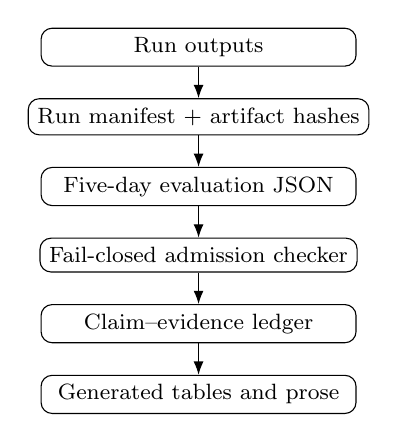
\begin{tikzpicture}[node distance=4mm, every node/.style={font=\footnotesize}, box/.style={draw,rounded corners,align=center,minimum width=40mm}, arr/.style={-Latex}]
\node[box] (run) {Run outputs};
\node[box,below=of run] (manifest) {Run manifest + artifact hashes};
\node[box,below=of manifest] (eval) {Five-day evaluation JSON};
\node[box,below=of eval] (gate) {Fail-closed admission checker};
\node[box,below=of gate] (ledger) {Claim--evidence ledger};
\node[box,below=of ledger] (paper) {Generated tables and prose};
\draw[arr] (run)--(manifest);\draw[arr] (manifest)--(eval);\draw[arr] (eval)--(gate);\draw[arr] (gate)--(ledger);\draw[arr] (ledger)--(paper);
\end{tikzpicture}
\caption{Evidence promotion path. Hash, schema, assertion, variant, contrast, or guardrail failure leaves a claim pending.}
\label{fig:evidence-flow}
\end{figure}

\begin{table}[t]
\caption{Claim status at manuscript generation time.}
\label{tab:claim-status}
\centering
\begin{tabular}{lr}
\toprule Status & Claims \\ \midrule
Verified & 15 \\
Preregistered & 3 \\
Pending & 10 \\
\bottomrule\end{tabular}
\end{table}


\section{Related Work}
TDM introduced expressive top-down tree retrieval for recommendation and considered tree learning~\citep{zhu2018tdm}. JTM formalized alternating optimization of index and preference model with hierarchical user representations~\citep{zhu2019jtm}. OTM analyzed mismatch between node-wise training and beam-search inference~\citep{zhuo2020otm}, while more recent DTR/TDR work emphasizes same-level multi-class competition and sampled softmax~\citep{liu2024dtr}. OTM's relevance-oriented pseudo-target and PTD's additive expected purchase-utility mass are different target constructions, but tree retrieval, horizontal competition, and finite-beam mismatch are prior art.

Knowledge distillation transfers behavior from a teacher into a deployable student~\citep{hinton2015kd}. Ranking-specific work studies listwise or top-ranked transfer~\citep{tang2018ranking,reddi2021rankdistil}, and Structural KD derives tractable local objectives when structured teacher and student factorizations agree, differ in granularity, or are incompatible~\citep{wang2021structural}. In text retrieval, RocketQAv2 dynamically couples a dense retriever and reranker with listwise distillation~\citep{ren2021rocketqav2}. Thus neither factorized KD nor ranker-to-retriever transfer is itself a PTD novelty.

Recommendation work has already established that independently trained nominators and rankers can interact poorly~\citep{hron2021components} and has transferred richer downstream objectives into candidate generation. DMTL distills click and reading-duration knowledge from a multi-task teacher into a candidate generator~\citep{zhao2021dmtl}; DMMP similarly transfers CTR/CVR knowledge into a multi-tower matching student~\citep{yi2024dmmp}. CoRR aligns recommendation retriever and ranker distributions through cooperative training and KL distillation~\citep{huang2023corr}, while Full Stage Learning to Rank propagates downstream selection preferences across a multi-stage system~\citep{zheng2024fsltr}. A multi-objective content-recall patent also describes distilling click/conversion outputs into an efficient recall model~\citep{tencent2025recall}. These works preclude claims that PTD is the first purchase-aware, conversion-aware, or downstream-aligned retriever distillation method.

Recent generative recommenders narrow the boundary further. OneMall uses an online ranker as a multi-objective reward for generative retrieval~\citep{zhang2026onemall}; BEAR and APAO explicitly optimize prefix survival under beam search~\citep{yang2026bear,yu2026apao}; SmartGR introduces hierarchy-aware and beam-aware distillation over semantic-ID generation~\citep{zhang2026smartgr}. PTD therefore does not claim the first hierarchical or beam-aware recommendation KD. Its registered distinction is the complete applied setting: item-level purchase utilities from a frozen downstream ranker are projected, through tree-induced descendant aggregation, onto sibling decisions of an upstream explicit tree retriever and evaluated under its serving-time finite-beam budget. ESMM supplies the frozen $pCTR\times pCVR$ score~\citep{ma2018esmm}, and HSTU supplies an encoder component~\citep{zhai2024hstu}; PTD modifies neither model.

\begin{table*}[!t]
\caption{Positioning against primary adjacent work. PTD statements describe the registered design, not empirical superiority.}
\label{tab:related}
\small
\begin{tabularx}{\textwidth}{l X X}
\toprule
Work & Prior mechanism & Registered PTD distinction \\
\midrule
TDM / JTM~\cite{zhu2018tdm,zhu2019jtm} & tree node / item leaf; teacher: none; tree: optional / alternating. & PTD retains coarse-to-fine retrieval and train-side reassignment but adds purchase-aware sibling targets from a frozen external ranker. \\
OTM / DTR~\cite{zhuo2020otm,liu2024dtr} & beam or same-level competing nodes; teacher: pseudo-target / none; tree: varies. & They address beam or horizontal competition; PTD transfers downstream purchase utility and treats finite-beam mismatch as residual. \\
Structural KD~\cite{wang2021structural} & structured output factors; teacher: structured predictor; tree: none. & Factorized KD and incompatible factorizations are prior art; PTD instantiates marginalization between heterogeneous funnel stages. \\
Funnel transfer~\cite{zhao2021dmtl,huang2023corr,yi2024dmmp,zheng2024fsltr,tencent2025recall} & candidate items or funnel stages; teacher: engagement, CTR-CVR, or downstream ranker; tree: none. & Ranker-to-retriever and conversion-aware alignment are prior art; PTD instantiates them at explicit tree-routing decisions. \\
OneMall / SmartGR~\cite{zhang2026onemall,yang2026bear,yu2026apao,zhang2026smartgr} & generated item or semantic-ID prefix; teacher: ranker reward / large generator; tree: semantic tokenizer. & Purchase rewards and hierarchy/beam-aware objectives are prior art; PTD evaluates tree-induced purchase-utility targets in an explicit index. \\
\bottomrule
\end{tabularx}
\end{table*}


\section{Limitations and Threats to Validity}
\paragraph{Construct validity.}
The ESMM score is a model-based proxy for purchase utility, not ground truth, user satisfaction, or welfare. It reflects historical exposure and can reproduce calibration, popularity, and representation biases. Internal-node mass is an expected utility/count mass over the frozen candidate universe, not a catalog-wide subtree probability. Moreover, leaf log-odds and internal additive mass form a hybrid local construction, not one globally consistent teacher factorization. The original registered ablations isolate item- and node-level signals but do not compare sum aggregation with max-descendant or binary-ancestor targets; causal attribution to the sum operator therefore remains pending on the separate mechanistic extension. Purchase NDCG emphasizes short-horizon conversion; the click, diversity, and concentration guardrails reduce but do not eliminate this mismatch.

\paragraph{Internal validity.}
The five test dates were used previously for legacy model evaluation, so the PTD analysis is prospective only with respect to the PTD readout, not blind to legacy outcomes. The tree also uses a fixed transductive envelope of test-period item identities and categories so that later items are representable; it never uses their labels or teacher scores, and this setup does not establish inductive new-item performance. Point-in-time assertions, fixed row keys, a frozen teacher, validation-only selection, immutable hashes, date masks, and a pre-test tree lock address identifiable leakage paths. They cannot rule out defects in upstream logging or unrecorded feature generation; a hash proves identity, not semantic correctness.

\paragraph{Statistical conclusion validity.}
Purchases are sparse and five date strata limit temporal replication. Pairing shared requests and seeds reduces variance but does not add dates. Holm correction covers only the four registered primary contrasts. Slice analyses, secondary outcomes, and the teacher oracle are descriptive; absence of significance is not evidence of equivalence.

\paragraph{External validity.}
One catalog, one historical teacher, a fixed tree family, and one beam/latency protocol limit generalization. Local sibling KL does not guarantee the globally best top-$K$ set under finite-beam pruning. Offline NDCG establishes neither online causal lift nor transfer to other catalogs and hardware. Until the five-day artifact is complete, this draft cannot support acceptance-level empirical conclusions; a positive result would still require a separately governed online experiment.

\section{Ethics and Societal Considerations}
Purchase optimization can over-emphasize high-propensity users or products, amplify exposure inequality, and encourage consumption. We record concentration and cold-start cohorts and forbid removal of failing slices. Private paired evidence uses access-controlled pseudonyms; the public artifact contains no row behavior. Review artifacts must be anonymous and policy compliant. Deployment requires separate safety and rollback review; an offline decision never changes production.

\section{Conclusion}
We specified Purchase-aware Tree Distillation as an applied combination of purchase-oriented ranker supervision and tree-induced marginalization for the sibling decisions of an explicit candidate retriever. The method uses additive expected descendant utility to create internal routing targets, while retaining teacher log-odds at leaves. The contribution is this heterogeneous funnel instantiation and its finite-beam evaluation, not factorized or marginal KD, downstream-objective alignment, hierarchy-aware KD, or beam-aware training in general. A separate prospective extension tests the stronger mechanism claim that aggregation controls early beam survival; the title and conclusions will not promote that claim unless the preregistered sum--beam--sparsity interactions and depth-wise mediation are reproduced. The artifact adds preregistered contrasts and a machine-checkable evidence boundary. \pending{Five-day PTD effect sizes, confidence intervals, latency measurements, and ablation conclusions await a valid artifact.}

\ifdefined\PTDAuthorVersion
\begin{acks}
This work was initiated during a one-month research visit to Fudan University.
\end{acks}
\fi

\FloatBarrier
\bibliographystyle{ACM-Reference-Format}
\bibliography{references}
\end{document}
